\section{Rumors on Twitter}
\begin{figure}[th]
\centering
\subfigure[09/29/14]{
   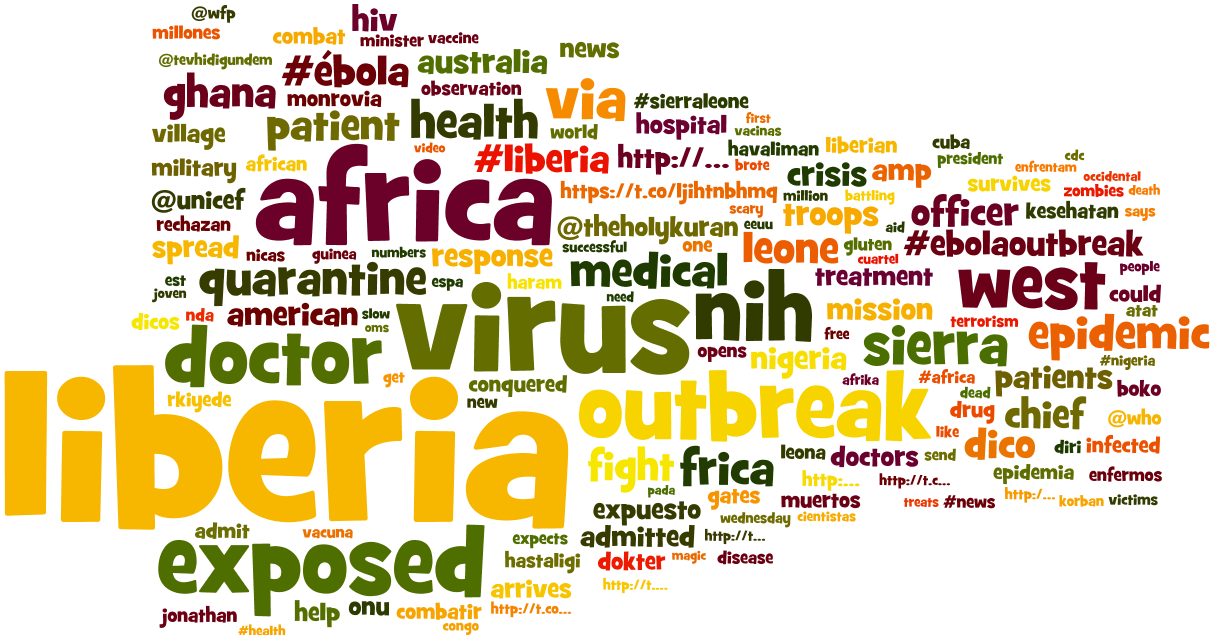
\includegraphics[width=2in,height=1.1in] {pictures/Word_cloud_0929.png}
  \label{fig:worldcloud29}
 }
 \subfigure[09/30/14]{
   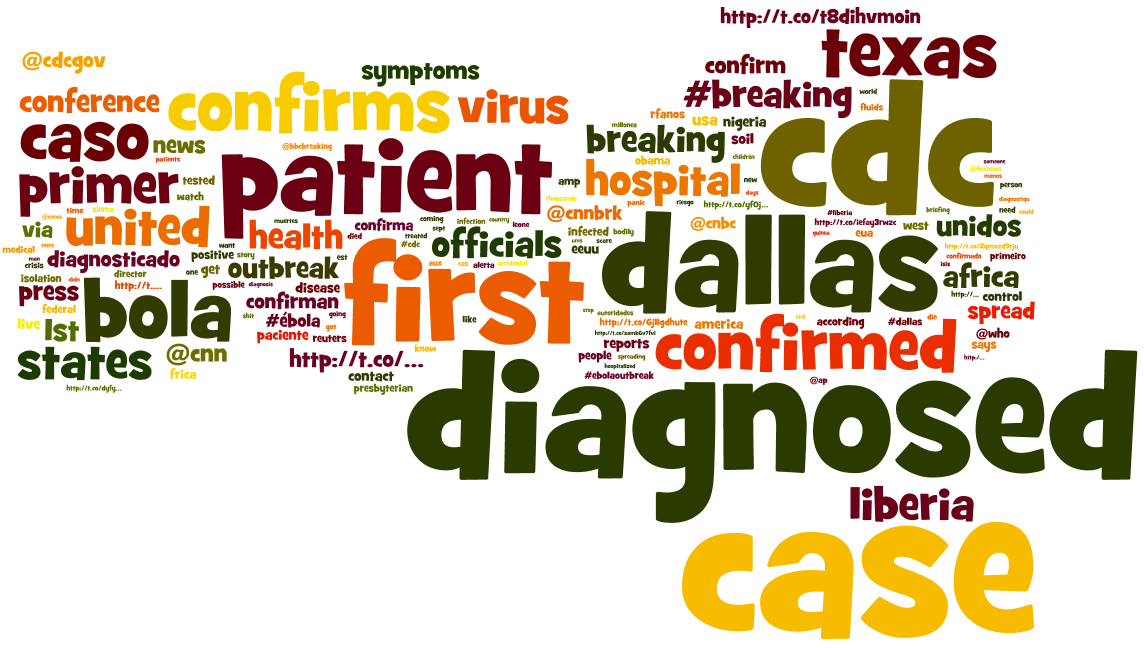
\includegraphics[width=2in,height=1.1in] {pictures/Word_cloud_0930.png}
  \label{fig:worldcloud30}
 }
 \subfigure[10/01/14]{
   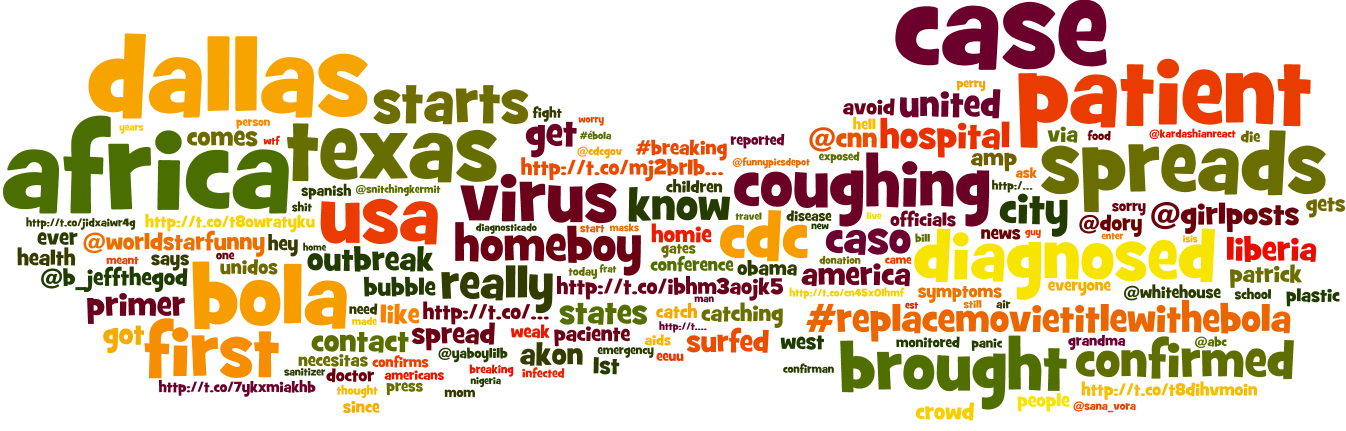
\includegraphics[width=2in,height=1.1in] {pictures/Word_cloud_1001.png}
  \label{fig:worldcloud01}
 }
\caption{Word clouds constructed from Ebola-related tweets.}
\label{fig:Ebola_word_cloud}
\end{figure}

The period from end of Sep to mid-late Oct, when Ebola activity happened in the US, is also the period when conspiracy theories, innuendo and rumors began to propagate wildly on Twitter. We gathered tweets during this period and filtered them by either the mention of the keyword `ebola' or relevant hashtags such as \#ebola, \#EbolaVirus, \#EbolaOutbreak, \#EbolaWatch, \#EbolaEthics, \#EbolaChat, \#nursesfightebola, \#ebolafacts, \#StopEbola, \#FightingEbola, and \#UHCRevolution.

From the gathered tweets, we removed stopwords for further processing. Figure~\ref{fig:Ebola_word_cloud} depicts word clouds constructed from the tweets for specific days. As can be seen, on 2014-09-29, when there was no Ebola incident in the US, people�s attention were primarily focused on Liberia and other African countries. On 2014-09-30, after CDC confirmed that Mr. Duncan in Dallas tested positive for Ebola, related keywords rose to the fore.


%Figure~\ref{fig:Ebola_time_series} depicts a simple frequency plot of specific keywords in Ebola-related tweets highlighting significant upticks for keywords such as Dallas, USA, CDC as well as �enfermera� (referring to the Spanish Nurse Romero and possibly other health professionals) during the studied period. Into mid October, we notice upticks in mentions of President Obama, likely due to proposed mitigation and response strategies by the US Government.
%
%
%\begin{figure}[ht]
%\centering
%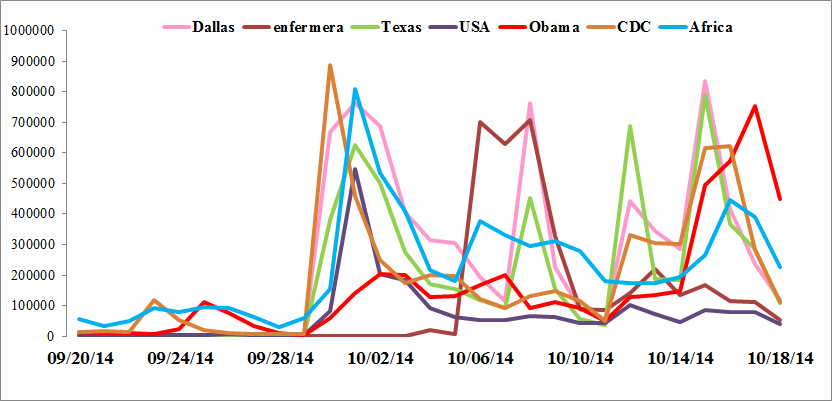
\includegraphics[width=5in]{pictures/time_series.png} %?????????????
%\caption{Frequency plot of specific keywords in Ebola-related tweets from 09/20/2014 to 10/18/2014}
%\label{fig:Ebola_time_series}
%\end{figure}

\begin{figure}[t]
\centering
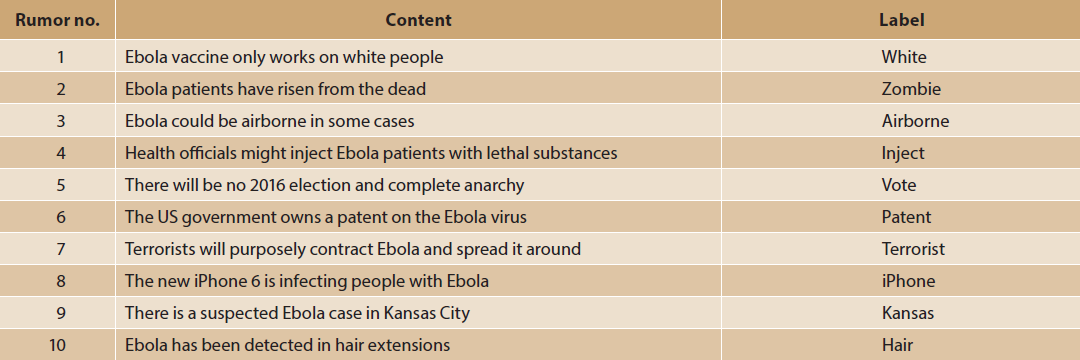
\includegraphics[width=6.5in, height=2.3in]{pictures/10_rumors_1.png} %?????????????
\caption{Top 10 Ebola-related rumors (by volume; from 09/28/2014 to 10/18/2014).}
\label{fig:Ebola_10rumors}
\end{figure}

\begin{figure}[ht]
\centering
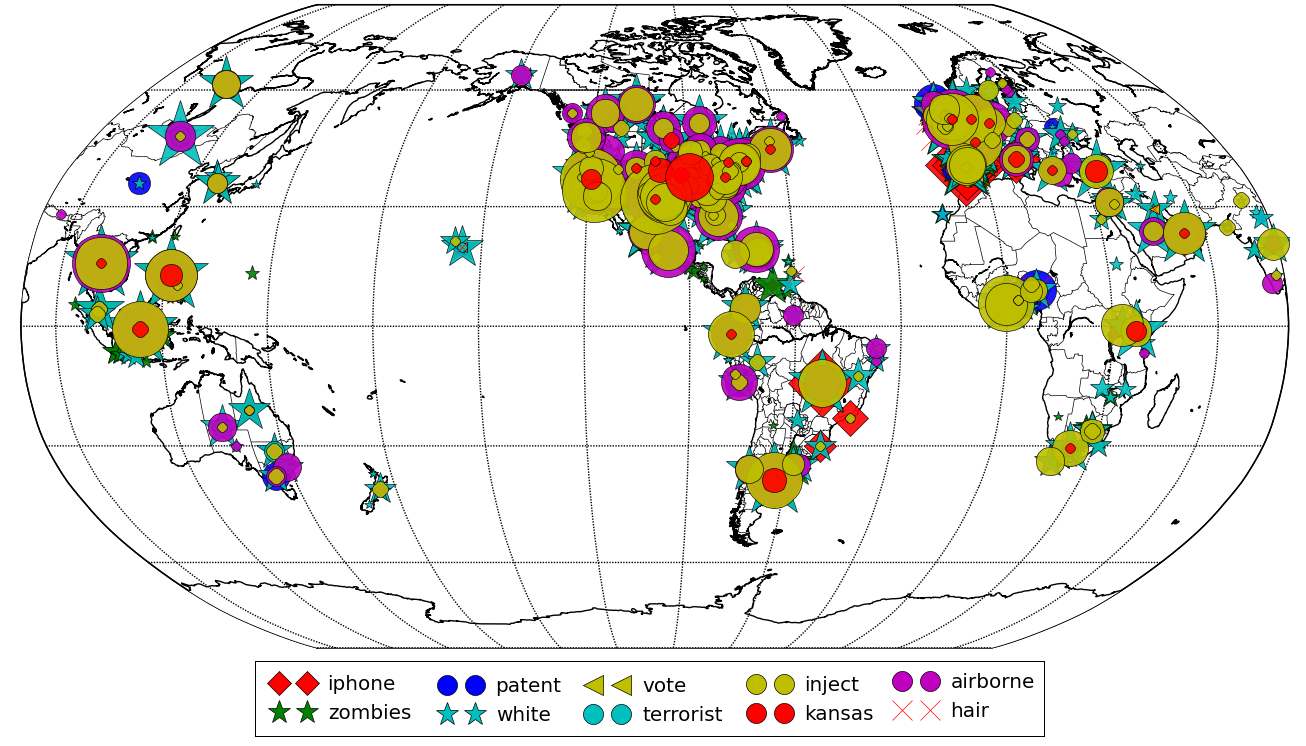
\includegraphics[width=5in]{pictures/20141008-map-country1.png} %?????????????
\caption{Distribution of top-10 rumors obtained from geolocated tweets. Data from 10/08/2014 is used for this plot. Icon size is proportional to the logarithm of the tweet volume.}
\label{fig:Ebola_map}
\end{figure}


Next, we studied information cascades in our collection of tweets with a view toward identifying misinformation and spread of falsehoods. We identified several widespread rumors circulating on Twitter, the top 10 of which are shown in Figure~\ref{fig:Ebola_10rumors}. (We focus on rumors in English only for our study.) Most are self-explanatory as to their intent and interpretation.


Two other rumors are note worthy. The `snake' rumor (which originated at least as early as late summer 2014) asserts that Ebola came across the border from Guinea to Sierra Leone via a snake in a bag. As stated in [4], ``a lady had a snake in a bag. When somebody opened the bag, that made the lady die.'' The Maldives rumor pertains to an uncorroborated report that Ebola patients have been reported (and quarantined) in the Maldives.

For each of these rumors, we geocoded tweets participating in the spread of such rumors with a view to understanding their geographical scope. As Figure~\ref{fig:Ebola_map} shows, the ``airborne'' and ``inject'' rumors were most prevalent in the US with specific other rumors (e.g., ``patent'') being prevalent in other parts of the world.



\begin{figure}[t]
\centering
\subfigure[09-29-2014]{
   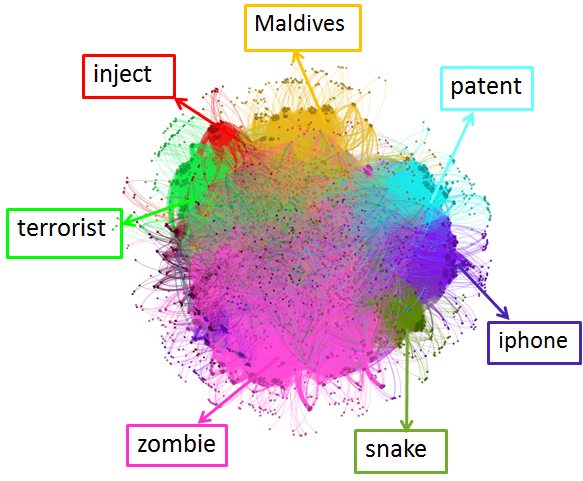
\includegraphics[width=3in] {pictures/rumor-cluster-20140929.png}
  \label{fig:worldcloud29}
 }
 \subfigure[10-06-2014]{
   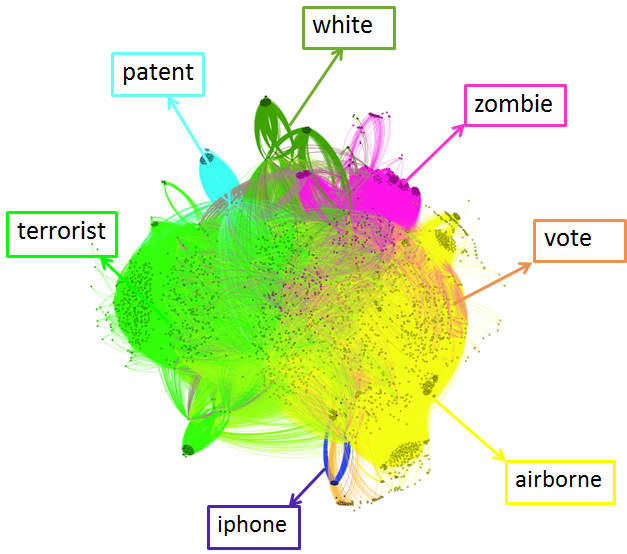
\includegraphics[width=3in] {pictures/rumor-cluster-20141006.png}
  \label{fig:worldcloud30}
 }
\caption{How rumors cluster: (a) 09/29/2014. (b) 10/06/2014. Rumors are color coded consistently across the two frames.}
\label{fig:Ebola_cluster}
\end{figure}

Next, we employed a dynamic query expansion model~\cite{zhao2014unsupervised} to study the rumors in greater detail. The DQE model begins with a seed set of keywords (e.g., ``ebola'', ``rumor''), identifies tweets that mentions these keywords, and iteratively expands them into a larger set of keywords. By conducting a modularity-based optimization over the underlying network of expanded tweets connected by shared keywords, DQE can identify specific localized instantiations of rumors.

As shown in Figure~\ref{fig:Ebola_cluster}, on 09/29/2014 (when there was no incidence of Ebola in the US), the dominant rumor is the zombie rumor. By 10/06/2014, other rumors pertaining to how Ebola can be airborne and that it is a potential terrorist weapon gained hold.



Although Figure~\ref{fig:Ebola_cluster} might suggest that rumors are quite rampant, it is important to keep in perspective that they are but a small fraction of all information propagation related to Twitter. Figure~\ref{fig:Ebola_patent_propagation} and~\ref{fig:Ebola_news_propagation} compare the time-indexed spread of the `patent' rumor versus a true news story (about the first US incidence of Ebola in Dallas). Here different colors denote different communities participating in information propagation, not different rumors/news stories. Each node in these graphs denotes a Twitter user, and an edge between nodes denotes a reply or retweet relationship. As can be seen, news stories permeate better whereas rumors are more localized, distributed, and comparatively smaller in permeation.

\begin{figure}[t]
\centering
\subfigure[09-30-2014]{
   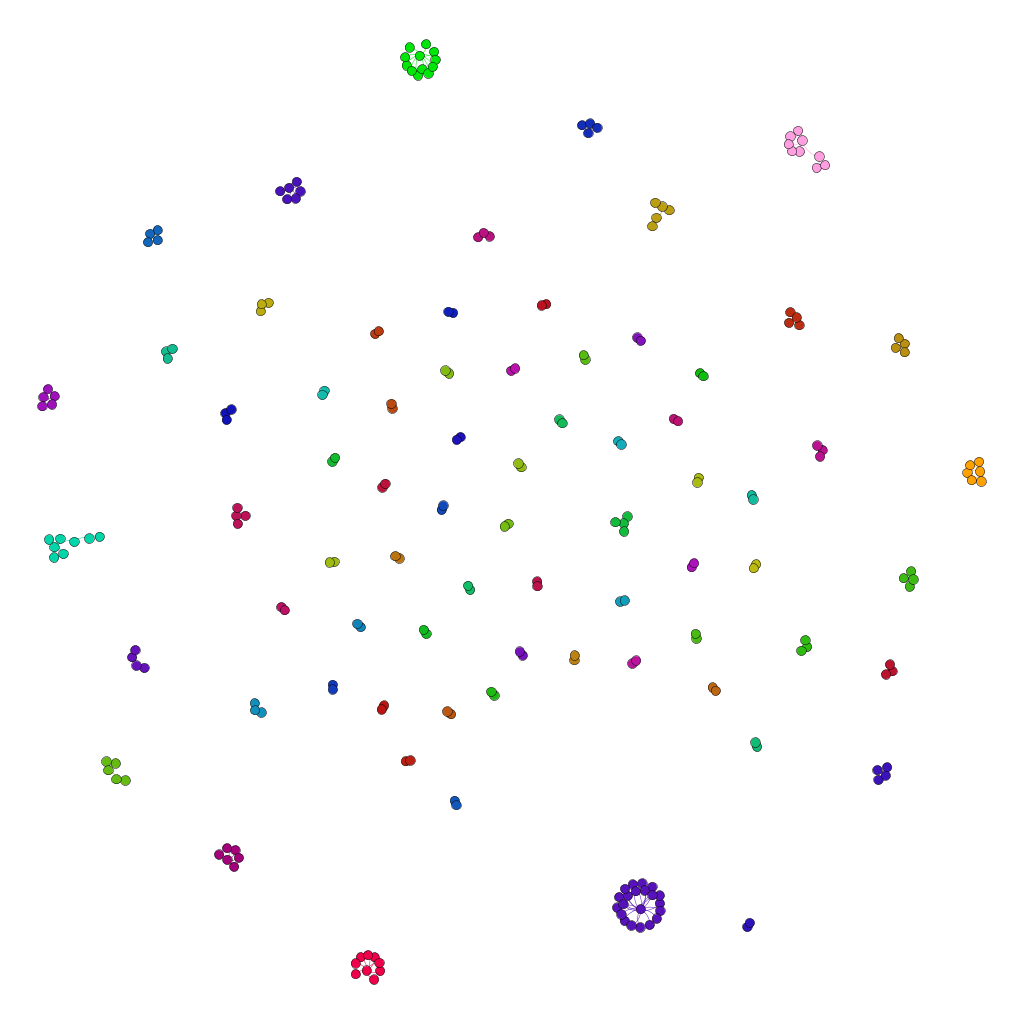
\includegraphics[width=2in] {pictures/patent_20140930.png}
  \label{fig:patent_20140930}
 }
 \subfigure[09-30-2014]{
   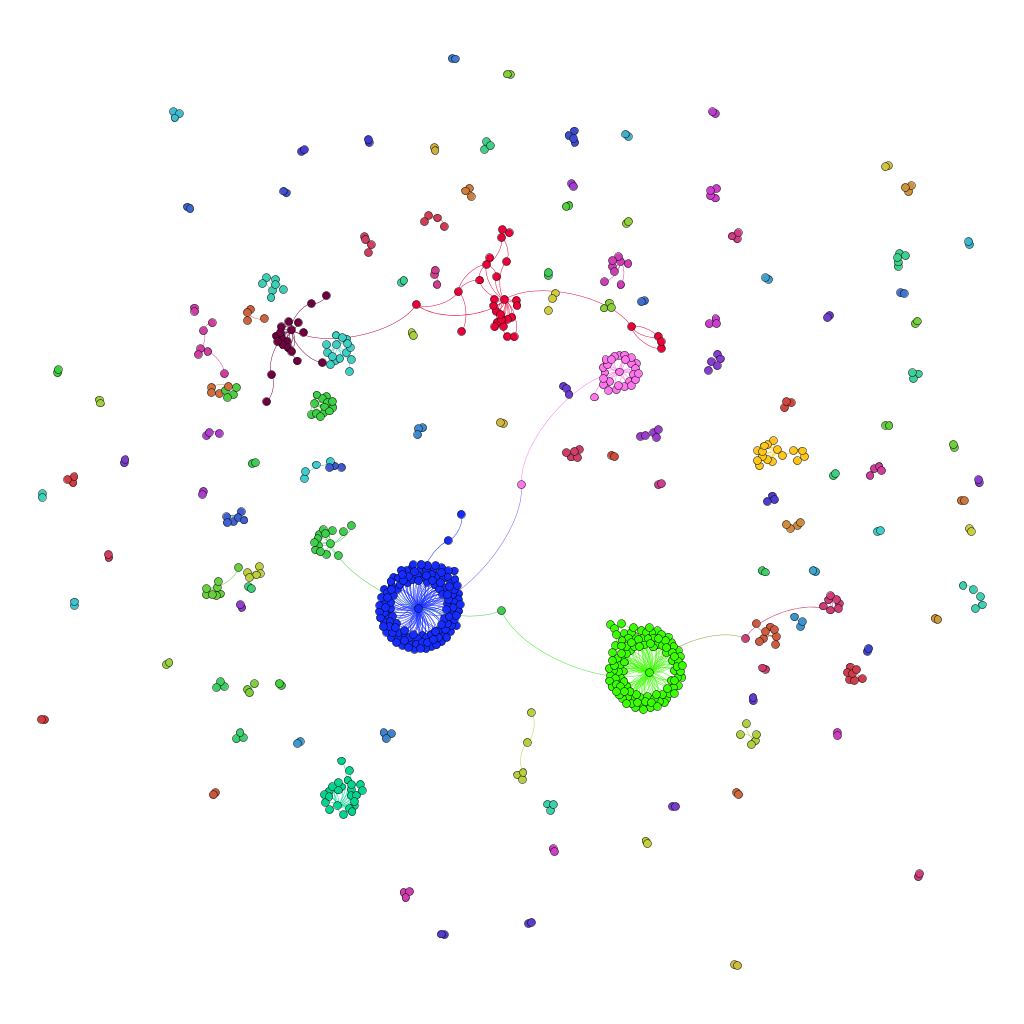
\includegraphics[width=2in] {pictures/patent_20141001.png}
  \label{fig:patent_20141001}
 }
 \subfigure[10-01-2014]{
   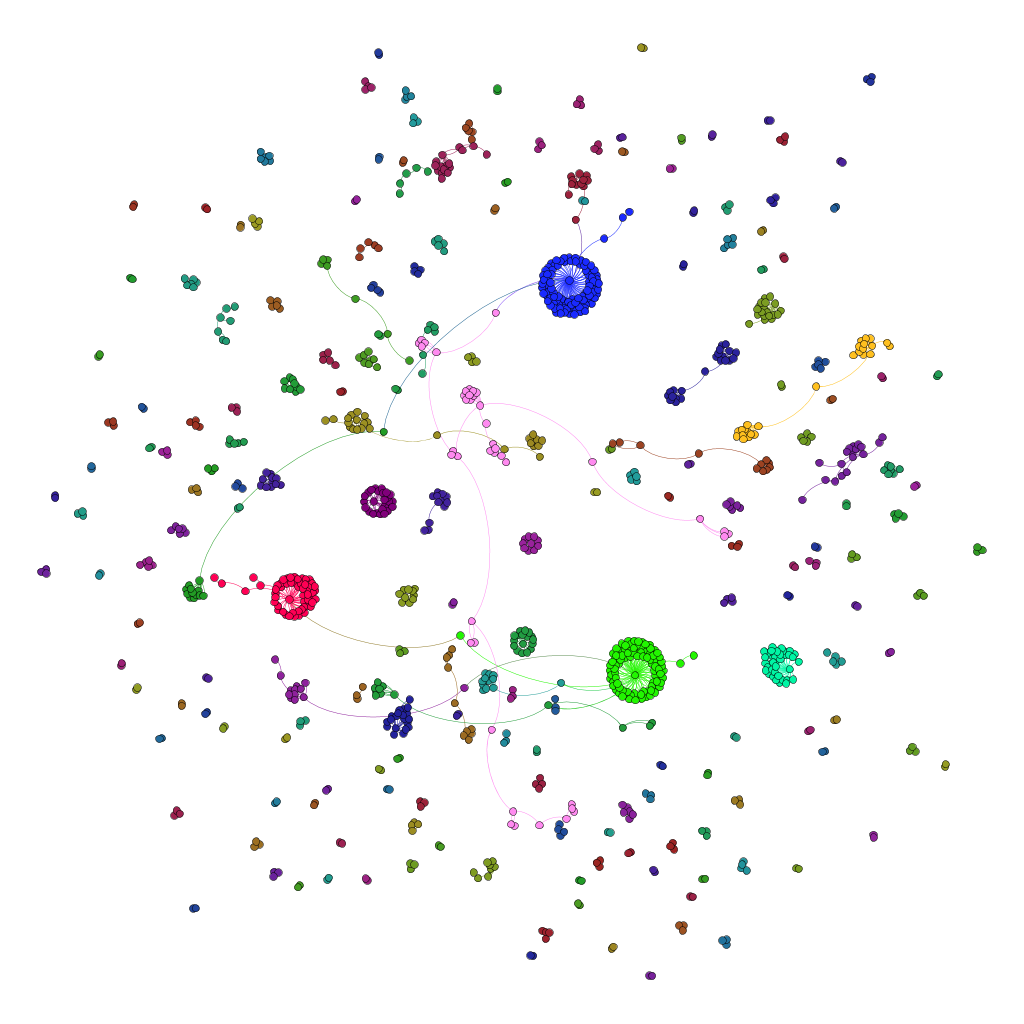
\includegraphics[width=2in] {pictures/patent_20141002.png}
  \label{fig:patent_20141002}
 }
\caption{Ebola-related patent rumor propagation over time.}
\label{fig:Ebola_patent_propagation}
\end{figure}



\begin{figure}[t]
\centering
\subfigure[09-30-2014]{
   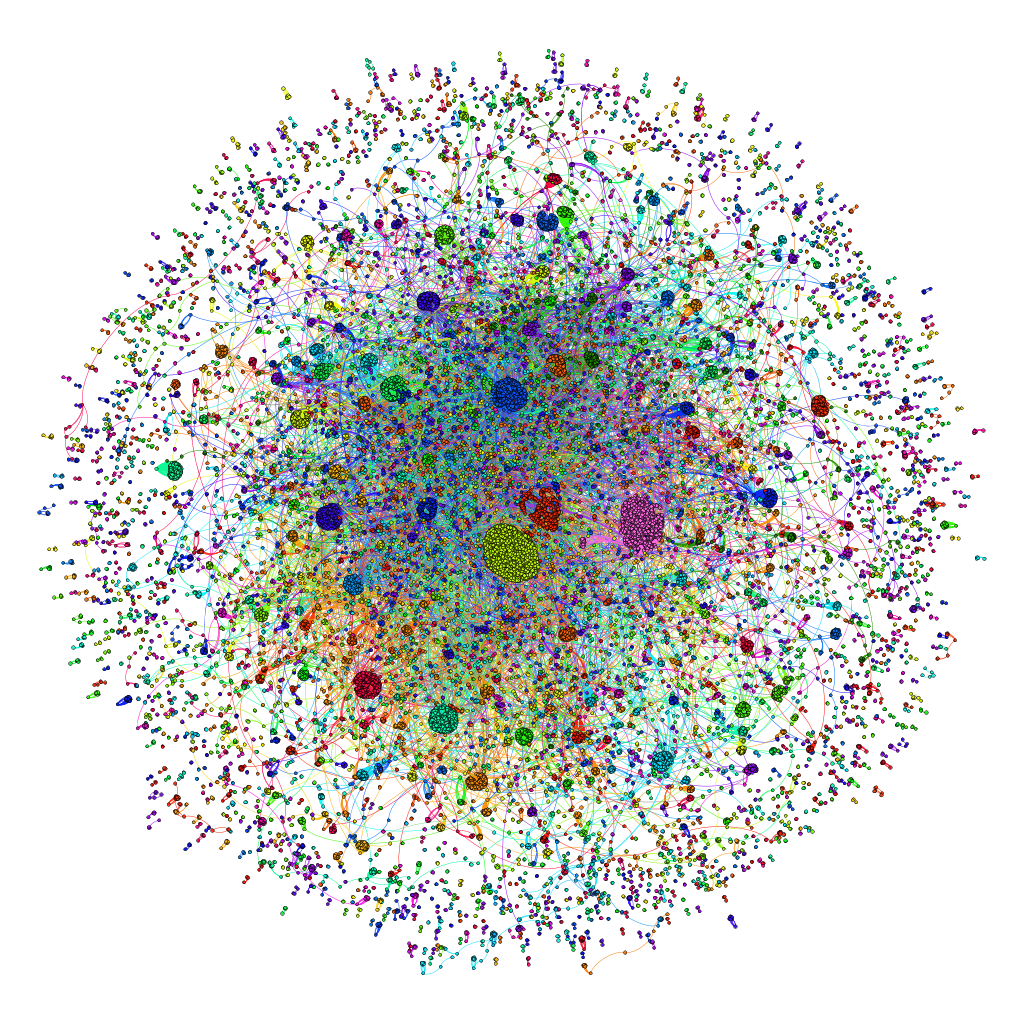
\includegraphics[width=2in] {pictures/dallas_20140930.png}
  \label{fig:dallas_20140930}
 }
 \subfigure[09-30-2014]{
   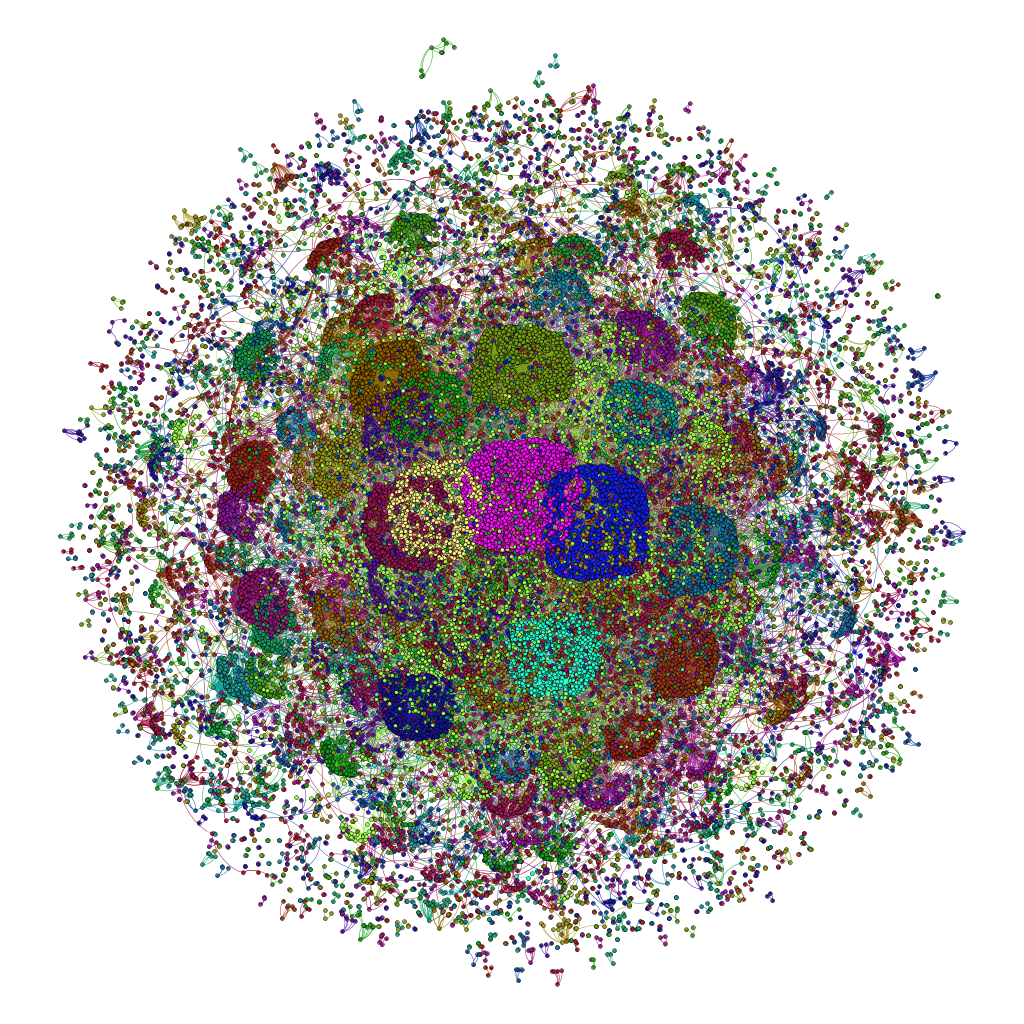
\includegraphics[width=2in] {pictures/dallas_20141001.png}
  \label{fig:dallas_20141001}
 }
 \subfigure[10-01-2014]{
   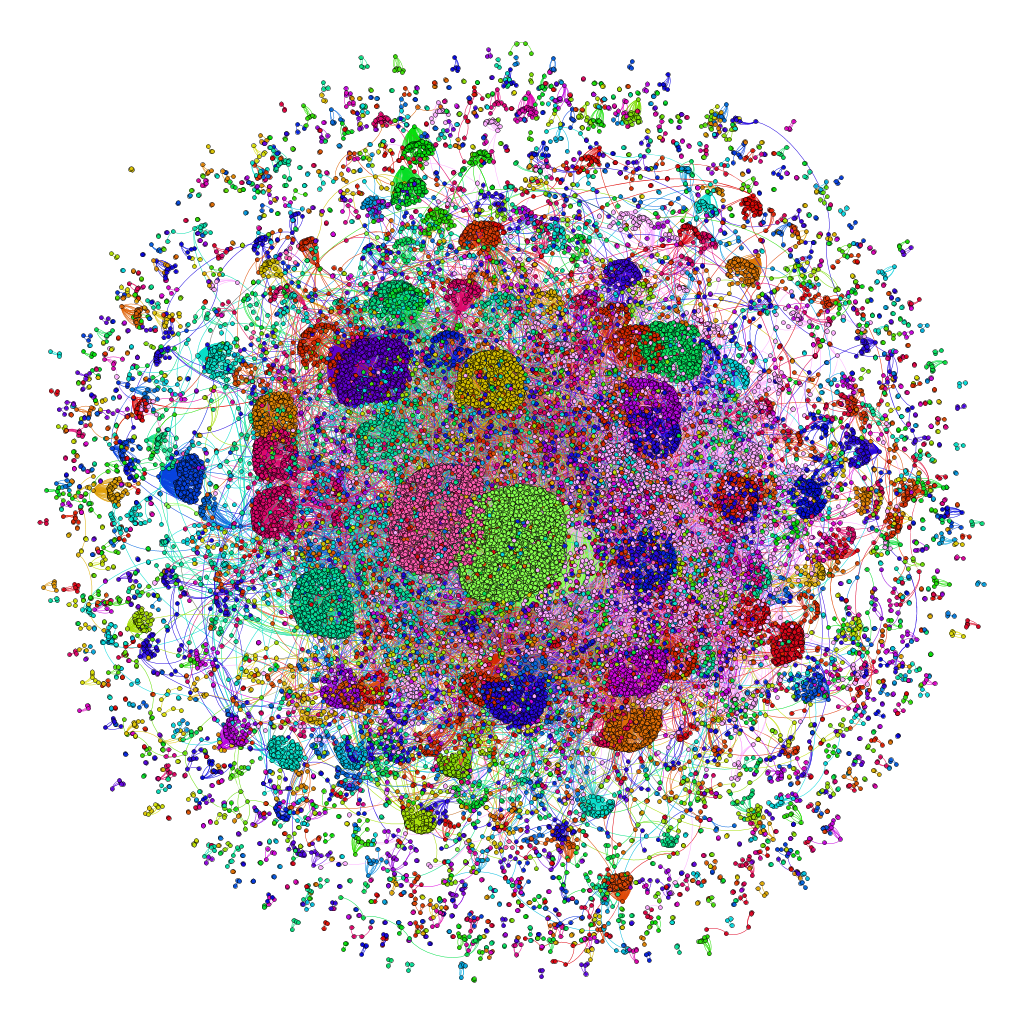
\includegraphics[width=2in] {pictures/dallas_20141002.png}
  \label{fig:dallas_20141002}
 }
\caption{Ebola-related Dallas news propagation over time.}
\label{fig:Ebola_news_propagation}
\end{figure}
